\documentclass{article}
\usepackage{graphicx}
\usepackage{physics}
\usepackage{amsmath}
\graphicspath{ {C:/Users/Peter/Desktop/} }

\begin{document}
\title{Project Optical Eigenmodes -- Three Wave Mixing in Fourier Space}
\author{ Peter Manshausen}
\date{19. September 2017}
\maketitle
\section{Introduction}
This project took place over the course of six weeks in the summer of 2017. It was an internship funded by the DAAD RISE worldwide scheme in the research group of Dr Michael Mazilu at the University of St Andrews. 
\\
\\
The aim of the project was to model nonlinear optical effects and to investigate possible ways towards Eigenfunctions (Eigenmodes) of a beam profile in a 2D nonlinear crystal. One of the simplest nonlinear effects is Three Wave Mixing whereby two rays of light interact to form a third one. 
\begin{figure}[h]
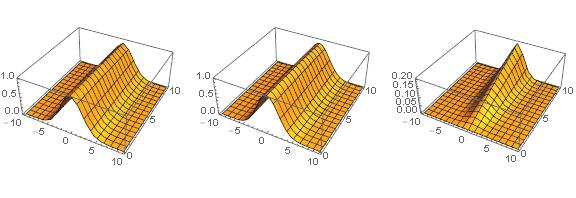
\includegraphics[width=\textwidth]{TWM}
\caption{An Example of Three Wave Mixing: Fields to the left and in the middle stay almost constant, the third field on the right is produced due to the nonlinear interaction. All units arbitrary.}
\end{figure}
This is used, for instance, in the everyday application of a green laserpointer. Two infrared waves interact, resulting in a visible -- green -- output. This interaction is not limited to the frequency domain. It also occurs in the spacial dimension of the beam profile. I tried to answer the question, whether for a given configuration of the input of the system, there would be a characteristic length ('interaction length') after which the input reproduces itself. This would then be very close to the properties of an 'Eigenmode' for a crystal of this length. 
\section{Model}
To model TWM, a 2D crystal with periodic boundary conditions  ($E(0)=E(x_{max})$) was described in Mathematica. I used the function NDSolve to numerically approximate the solution to the differential equations governing the system. These are the following three coupled partial differential equations -- the Manley-Rowe-Relations:
 \begin{equation}
\frac{\partial E_1} {\partial z}=-\frac{i}{2k_1} \pdv [2]{E_1}{x}-\frac{i \omega_1}{2 c n_1} \chi^{(2)}E_3 E_2^*e^{-i\Delta k z}
\end{equation}
\begin{equation}
\frac{\partial E_2} {\partial z}=-\frac{i}{2k_2} \pdv [2]{E_2}{x}-\frac{i \omega_2}{2 c n_2} \chi^{(2)}E_3 E_1^*e^{-i\Delta k z}
\end{equation}
\begin{equation}
\frac{\partial E_3} {\partial z}=-\frac{i}{2k_3} \pdv [2]{E_3}{x}-\frac{i \omega_3}{2 c n_3} \chi^{(2)}E_1 E_2 e^{i\Delta k z}
\end{equation}
where $E_i$ describes the ith field of angular frequency $\omega_i$, wavenumber $k_i$ and refraction index $n_i$, $z$ is the direction of propagation, $x$ the transversal direction and $\chi^{(2)}$ the nonlinear susceptibility tensor of rank two giving the strength of the fields' interaction.The exponential term fulfills $\Delta k= k_3-k_2-k_1$, the frequencies relate via $\omega_3=\omega_1+\omega_2$. A good test of whether the model is working is to look at energy conservation: Fig. 2 shows a plot demonstrating constant total energy even as the absolute values of the fields vary. 
\begin{figure}[h]
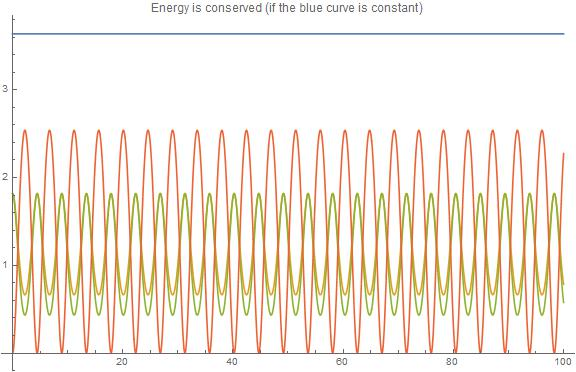
\includegraphics[scale=0.4]{energyconservation}
\caption{Conservation of energy: The blue line at the top shows the evolution of total energy to be constant while the absolute values of the fields show a periodically varying behaviour.}
\end{figure}
More specifically, my project looked at input functions whose spatial profile was given by a set of Fourier modes, such that
$$E_i(z)= \sum_{n=-N}^{N} a_{i,n}(z) \exp(n \frac{2\pi x}{x_{max}})$$
The question about the form of the output function is the the question about the evolution of the coefficient functions $a_{i,n}(z)$. Is there an interaction length, after which they will be (almost) as in the beginning? Plugging into the Manley-Rowe-relations yields: 
\begin{equation}
k_1 i\frac{\partial a_{1, n}} {\partial z}=\frac{1}{2}(\frac{n 2 \pi}{x_{max}})^2 a_{1, n}-\frac{\chi^{(2)} \omega_1^2}{c^2}  e^{-i\Delta k z} \sum_{m=-N}^{N} a_{2, m}^* a_{3, n+m}
\end{equation}
\begin{equation}
k_2 i\frac{\partial a_{2, n}} {\partial z}=\frac{1}{2}(\frac{n 2 \pi}{x_{max}})^2 a_{2, n}-\frac{\chi^{(2)} \omega_2^2}{c^2} e^{-i\Delta k z} \sum_{m=-N}^{N} a_{1, m}^* a_{3, n+m} 
\end{equation}
\begin{equation}
k_3 i\frac{\partial a_{3, n}} {\partial z}=\frac{1}{2}(\frac{n 2 \pi}{x_{max}})^2 a_{3, n}-\frac{\chi^{(2)} \omega_3^2}{c^2} e^{i\Delta k z} \sum_{m=-N}^{N} a_{1, m} a_{2, n-m}. 
\end{equation}
where, interestingly, the multiplication becomes a convolution (the sums at the end of the right hand sides), this being predicted by the convolution theorem. From the equations, we find a symmetry concerning the complex phases of the coefficients: The equations are invariant under the transformation 
$$a_{1, n} \longrightarrow a_{1, n} \exp(i \phi_1)$$
$$a_{2, n} \longrightarrow a_{2, n} \exp(i \phi_2)$$
$$a_{1, n} \longrightarrow a_{3, n} \exp(i \phi_3)$$
$$where \ \phi_3=\phi_1+\phi_2.$$
We are therefore not necessarily interested in coefficients \emph{exactly} replicating initial values, but allow for a common phase of $E_i$ coefficients for each i under the condition that those of the first and the second add up to the third. This allows us to define an error function which gives out the deviation from the desired value configuration as a function of the propagation distance.
\begin{align}
\nonumber f(z)=\sum_{i=1}^{3}\bigg(\sum_{n} (\abs{a_{i, n}(z)} -\abs{a_{i, n}(0)})^2+(\bigl|\sum_n a_{i, n}(z) a_{i, n}^*(0) \bigr|-\sum_n\abs{ a_{i, n}(z) a_{i, n}^*(0)})^2\bigg) \\ +\ (\Im(a_{1,1}(z) a_{2,1}(z) a_{3,1}^*(z))-\Im(a_{1,1}(0) a_{2,1}(0) a_{3,1}^*(0)))^2
\end{align}
Here, the first squared term checks for the absolute values of the coefficients being equal, the second one, whether within one field, the phase of the coefficients are the same and the third one, whether the condition  $\phi_3=\phi_1+\phi_2$ is met. Because all terms are non-negative, the function goes to zero if and only if every term is equal to zero.

\section{Example}
For illustration, we can look at the following input: Modes in $E_1$: $n=4 \ and \ 5$ and $E_2$: $n=3\ and \ 4$, length of crystal in transversal direction: 10, length of crystal in transversal direction: 50, angular frequencies $\omega_1=\omega_2=5$, refraction indices $n_1=n_2=1,5$, $n_3=1,6$. This corresponds to the midde picture in Fig. 3. Numerically, we find a promising zero of the function at $z=31,3109$. The coefficients are given in the following table.
\begin{center}
 \begin{tabular}{||c c c c||} 
 \hline
Field & Fourier mode n & absolute value & Input absolute value \\ [0.5ex] 
 \hline\hline
 1 & 4 & 0.78 &  0.78 \\ 
 \hline
 1 & 5 & 0.78 &  0.78 \\
 \hline
 2 & 3 & 0.78 &  0.78 \\
 \hline
 2 & 4 & 0.78 &  0.78 \\
 \hline
 3 & 7 & 0.01 &  0.00 \\
 \hline
 3 & 8 & 0.01 &  0.00 \\
 \hline
 3 & 9 & 0.01 &  0.00 \\ [1ex] 
 \hline
\end{tabular}
\end{center}
Input is reproduced well here. The errorfunction also guarantees reproduction of phase, which I have omitted here for briefness.
\section{Results}
Indeed, exact periodicity within the numerical error of the programme is achieved for those configurations, where the input fields consist of only one mode. The more modes are added, the larger the interaction length becomes, after which we obtain approximate zeros of the error function. This makes sense, as each mode will have its own periodic behaviour and the errorfunction will only go to zero when all of the periods coincide. Fig. 3 shows the evolution of the error function in the cases of one, two and three Fourier modes, respectively.
\begin{figure}[h]
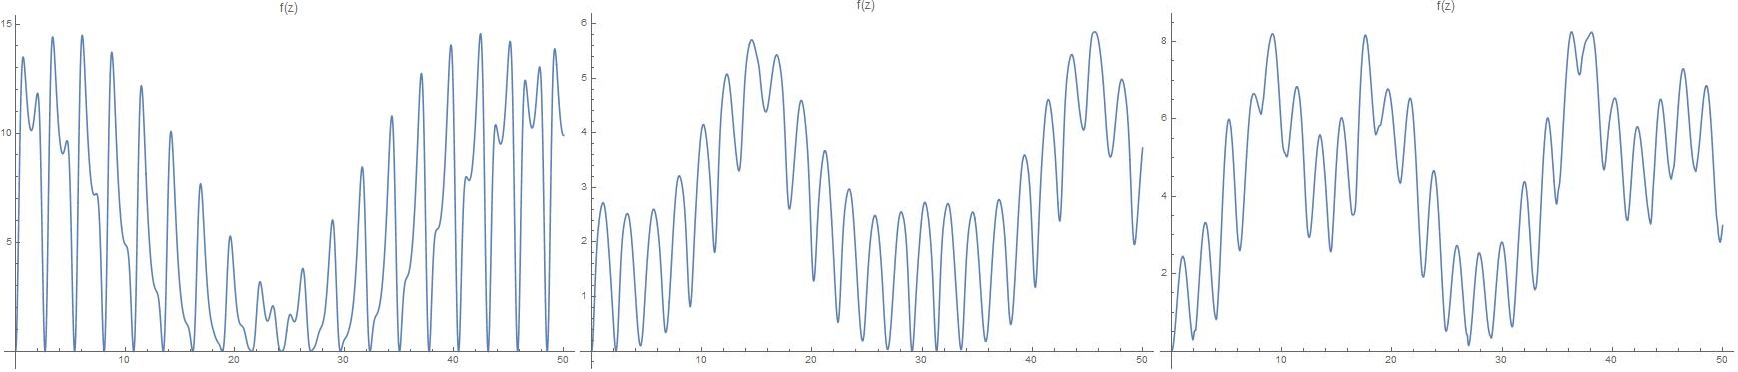
\includegraphics[width=\textwidth]{allthree}
\caption{Error function: From left to right with the input of one, two and three Fouriermodes, starting with a Gaussian distribution of absolute values for each field. All units arbitrary.}
\end{figure}
The biggest determining factor for the interaction length, besides the number of input modes, seems to be the susceptibility tensor $\chi^{(2)}$. If an interaction length is indeed discernible, $\chi^{(2)}$ is nearly inversely proportional to it. This makes sense, when we consider this value determining the strength of the nonlinearity and thereby the interaction of the different fields.
\section{Conclusion and way forward}
The results show that the ansatz of decompostion into Fourier modes is a good idea, with the limitation that a larger number of those tend to make the system chaotic. This is intimately related to the nature of the problem: While usually, Fourier decomposition allows to seperate the modes from each other and propagate them forward independently, this is not possible in a nonlinear problem. Waves do not just add up (superposition) but influene each other. It would therefore be advisable to continue the research by first only looking at single Fourier modes. Interesting questions include the role of system parameters $\chi^{(2)}, \omega_i, \Delta k, n_i$. Also, in the end, the goal would be to not look for an interaction length given a specific input, but to look for a input given a fixed length of the crystal, which is supposed to reproduce itself. This would be one step closer to a proper 'Eigenmode' of the system.
\\
\\
I would like to thank Dr Mazilu, Graeme Docherty-Walthew and DAAD for the insights gained from this project and for the opportunity to carry out this internship.
\end{document}